\documentclass[a4paper,10pt]{article}

\usepackage[margin=2cm, tmargin=1.5in, headheight=40px]{geometry}
\usepackage[sfdefault, medium, light]{roboto}
%\usepackage[nomap]{FiraMono}
\usepackage[T1]{fontenc}
\usepackage[utf8]{inputenc}
\usepackage[spanish]{babel}
\usepackage{graphicx}
\usepackage{fancyhdr}
\usepackage{minted}
\usepackage[svgnames]{xcolor}
\setminted{style=default,bgcolor=Gainsboro}
\usepackage[allcolors={DarkSlateBlue}, colorlinks]{hyperref}

\fancyhf{}
\fancyhead[L]{
\includegraphics[height=35px]{../figuras/logoort.png}}
\fancyhead[R]{Facultad de Ingeniería \\ Cátedra de Redes y Sistemas de Comunicación}
\fancyfoot[R]{Página \thepage}
\fancyfoot[L]{Redes -- Laboratorio 6}
\renewcommand{\footrulewidth}{0.2pt}
\renewcommand{\headrulewidth}{0.2pt}

\pagestyle{fancy}


\title{\bf Redes\\Laboratorio 6 -- Capa de Enlace}
\author{\bf Universidad ORT Uruguay}
\date{\bf Curso 2026}

\begin{document}

\maketitle
\thispagestyle{fancy}

En este laboratorio trabajaremos a nivel de Capas de Red y de Enlace, utilizando una topología de Red definida en el simulador GNS3. La idea es que la topología simula una red de acceso conformada por una LAN con varios switches y PC y un servidor alojado en una red remota.

Los objetivos de este laboratorio son:

\begin{itemize}
    \item Observar el intercambio DHCP para lograr la auto-configuración de las interfaces de red en una LAN.
    \item Lograr conectividad entre varias LAN a través de Routers y Switches.
    \item Observar el comportamiento del protocolo ARP para mapear direcciones de capa de red en direcciones de capa de enlace.
    \item Cómo se usan estas direcciones de capa de enlace para la comunicación local.
\end{itemize}

La topología base del laboratorio es la siguiente:

\bigskip

\begin{center}
    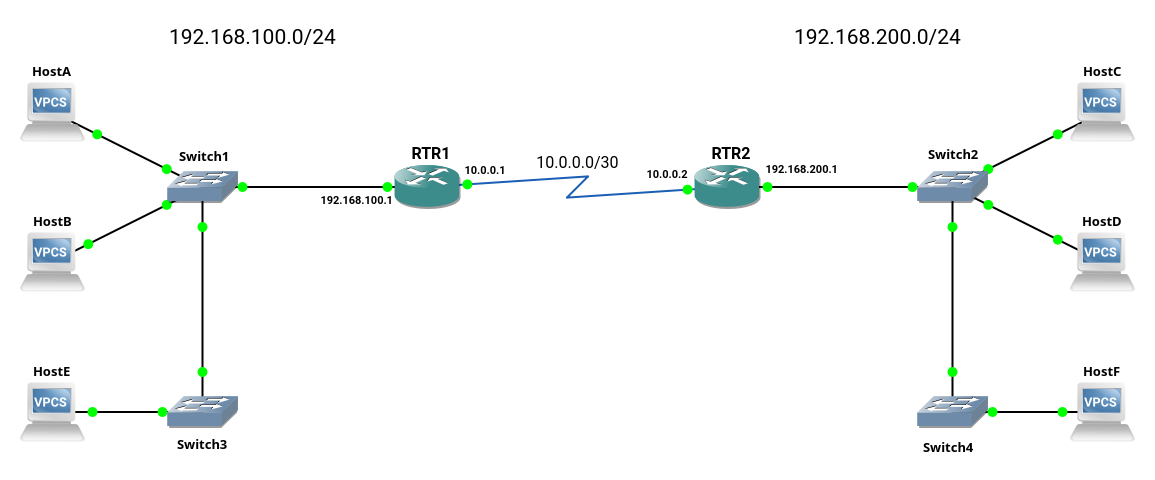
\includegraphics[width=0.9\textwidth]{../figuras/topologia_lab6.png}
\end{center}

\section{Preparación}

Antes de comenzar la práctica:

\begin{enumerate}
    \item Importe el proyecto portable GNS3 \texttt{topologia-lab-6.gns3project}.
    \item Inicie la simulación encendiendo todos los equipos.
    \item Verifique con \mintinline{batch}{# show ip interface brief} y \mintinline{batch}{# show ip route} que los routers están adecuadamente configurados, tienen las rutas correctas y las interfaces levantadas. Pruebe hacer \texttt{ping} entre ellos.
    \item Ingrese a una consola del Servidor y verifique que tiene su ip asignadda con \mintinline{batch}{Servidor> show ip}. Pruebe hacer \texttt{ping} a los routers.
\end{enumerate}

Al terminar esta parte, los PCs no tienen su capa de red configurada y no pueden acceder a la red.

\section{Protocolo DHCP}

En esta parte, configuraremos al Router RTR1 para que actúe como servidor DHCP de la LAN.

\begin{enumerate}
    \item Inicie una consola al router RTR1 e introduzca la siguiente configuración:
    \begin{minted}{batch}
    RTR1# configure terminal
    RTR1(config)# ip dhcp pool LAN
    RTR1(dhcp-config)# network 192.168.100.0 255.255.255.0
    RTR1(dhcp-config)# default-router 192.168.100.1
    RTR1(dhcp-config)# exit
    RTR1(config)# ip dhcp excluded-address 192.168.100.1
    \end{minted}

    Esta configuración le permite al router contestar pedidos DHCP en un pool de direcciones llamado LAN, en la red indicada. Además indica que él es el default-router de la red, por lo que las PCs tendrán una ruta por defecto en la autoconfiguración. Finalmente, se excluye la IP propia del pool.

    \item Comience a capturar paquetes en la interfaz HostA - Switch1 utilizando Wireshark (click derecho en el link y comenzar captura).
    \item Inicie una consola a la PC HostA y habilite la autoconfiguración DHCP utilizando \mintinline{batch}{HostA> ip dhcp}
    \begin{enumerate}
     \item ¿Logra ver un intercambio de autoconfiguración en la captura? Analice el mismo.
     \item ¿La IP asignada es válida para el rango? Tome nota de su valor y por cuánto tiempo es válida.
     \item Verifique en el HostA con \mintinline{batch}{HostA> show ip} que el host quedó correctamente configurado.
     \item ¿Puede hacer ping al servidor ahora?
    \end{enumerate}

    \item Repita los pasos anteriores de configuración para los HostB y HostC, y tome nota de las IP asignadas a cada uno.
    \item Realice una prueba de conectividad mediante \texttt{ping} a otra PC de su misma LAN. ¿Es exitoso?
    \item Realice una prueba de conectividad mediante \texttt{ping} al Router de su LAN. ¿Es exitoso?
\end{enumerate}

\bigskip
\textbf{Preguntas adicionales para discutir:}

\begin{itemize}
    \item ¿Por qué es necesario un servidor DHCP para cada LAN, y no puede resolverse el problema con un único servidor DHCP global?
    \item ¿Qué podría ocurrir si una PC configura de manera \emph{estática} una dirección que ya fue asignada a otra por DHCP?
    \item ¿Cómo podría usar un servidor DHCP malicioso para interceptar el tráfico de los usuarios de una LAN?
\end{itemize}

\section{Protocolo ARP}

Antes de comenzar esta parte, en la consola de las PCs utilice el comando \mintinline{batch}{HostA> clear arp} para borrar la tabla ARP. Puede chequear en cualquier momento el estado actual de la tabla con \mintinline{batch}{> show arp}.

\begin{enumerate}
    \item Comience nuevamente a capturar tráfico en la interfaz de red del HostA.
    \item Realice un \texttt{ping} al Router de su LAN. ¿Qué ocurre antes de que se envíe el paquete ICMP request? ¿Ocurre algo similar con el ICMP reply? ¿Por qué?
    \item Realice un \texttt{ping} a otra PC cualquiera de su misma LAN.
        \begin{enumerate}
            \item ¿Logra ver un intercambio ARP? ¿Por qué es necesario esto?
            \item Tome nota de las direcciones IP origen y destino de los paquetes, así como de las direcciones MAC origen y destino. ¿A qué dispositivos corresponden?
        \end{enumerate}
    \item Verifique el estado de la tabla ARP de su máquina al finalizar estos intercambios.
    \item Realice un \texttt{ping} a otra PC cualquiera de la otra LAN.
        \begin{enumerate}
            \item ¿Logra ver un intercambio ARP? ¿Es necesario esto? Chequee si ya dispone de las MAC adecuadas en su tabla ARP.
            \item Tome nota de las direcciones IP origen y destino de los paquetes, así como de las direcciones MAC origen y destino. ¿A qué dispositivos corresponden?
            \item ¿Su PC requiere conocer la dirección MAC de la PC destino del \texttt{ping}?
        \end{enumerate}
\end{enumerate}

\bigskip

\textbf{Preguntas adicionales para discutir:}

\begin{itemize}
    \item ¿Cuál es el rol que cumplen las direcciones MAC, si ya existen las IP?
    \item ¿Por qué los Switches no necesitan tener una dirección IP asignada?
    \item ¿Los Switches tienen tabla ARP?
    \item ¿Cómo saben los Switches a dónde deben redirigir los paquetes, si no poseen una tabla de rutas?
\end{itemize}


\end{document}